\begin{figure}[h!]
	\centering

	
	
	\tikzset{every picture/.style={line width=0.75pt}} %set default line width to 0.75pt        
	
	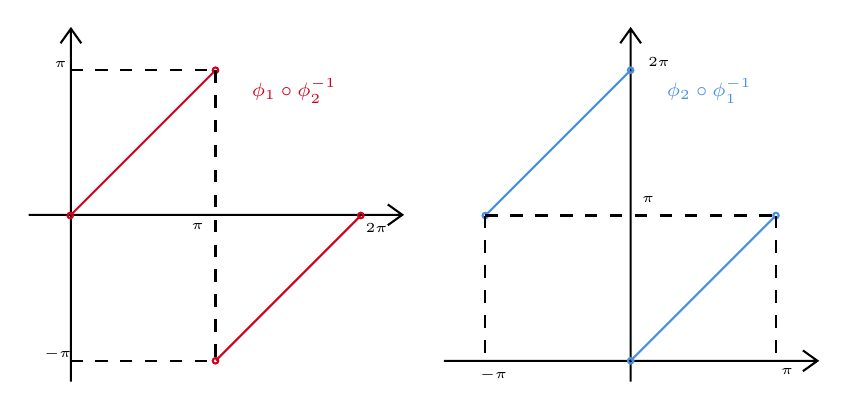
\begin{tikzpicture}[x=0.75pt,y=0.75pt,yscale=-1,xscale=1]
		%uncomment if require: \path (0,300); %set diagram left start at 0, and has height of 300
		
		%Shape: Axis 2D [id:dp031269396086308854] 
		\draw  (180,189.67) -- (360,189.67)(200.33,100) -- (200.33,270) (353,184.67) -- (360,189.67) -- (353,194.67) (195.33,107) -- (200.33,100) -- (205.33,107)  ;
		%Straight Lines [id:da8173483474090752] 
		\draw [color={rgb, 255:red, 208; green, 2; blue, 27 }  ,draw opacity=1 ][line width=0.75]    (200.24,189.76) -- (269.76,120.24) ;
		\draw [shift={(270,120)}, rotate = 315] [color={rgb, 255:red, 208; green, 2; blue, 27 }  ,draw opacity=1 ][line width=0.75]      (0, 0) circle [x radius= 1.34, y radius= 1.34]   ;
		\draw [shift={(200,190)}, rotate = 315] [color={rgb, 255:red, 208; green, 2; blue, 27 }  ,draw opacity=1 ][line width=0.75]      (0, 0) circle [x radius= 1.34, y radius= 1.34]   ;
		%Straight Lines [id:da7972743834901372] 
		\draw [color={rgb, 255:red, 208; green, 2; blue, 27 }  ,draw opacity=1 ][line width=0.75]    (270.24,259.76) -- (339.76,190.24) ;
		\draw [shift={(340,190)}, rotate = 315] [color={rgb, 255:red, 208; green, 2; blue, 27 }  ,draw opacity=1 ][line width=0.75]      (0, 0) circle [x radius= 1.34, y radius= 1.34]   ;
		\draw [shift={(270,260)}, rotate = 315] [color={rgb, 255:red, 208; green, 2; blue, 27 }  ,draw opacity=1 ][line width=0.75]      (0, 0) circle [x radius= 1.34, y radius= 1.34]   ;
		%Straight Lines [id:da11749218813373297] 
		\draw  [dash pattern={on 4.5pt off 4.5pt}]  (270,120) -- (270,260) ;
		%Shape: Axis 2D [id:dp7242837319994968] 
		\draw  (380,260) -- (560,260)(470,100) -- (470,270) (553,255) -- (560,260) -- (553,265) (465,107) -- (470,100) -- (475,107)  ;
		%Straight Lines [id:da7954245800299584] 
		\draw [color={rgb, 255:red, 74; green, 144; blue, 226 }  ,draw opacity=1 ][line width=0.75]    (400.24,189.76) -- (469.76,120.24) ;
		\draw [shift={(470,120)}, rotate = 315] [color={rgb, 255:red, 74; green, 144; blue, 226 }  ,draw opacity=1 ][line width=0.75]      (0, 0) circle [x radius= 1.34, y radius= 1.34]   ;
		\draw [shift={(400,190)}, rotate = 315] [color={rgb, 255:red, 74; green, 144; blue, 226 }  ,draw opacity=1 ][line width=0.75]      (0, 0) circle [x radius= 1.34, y radius= 1.34]   ;
		%Straight Lines [id:da15608839189923596] 
		\draw [color={rgb, 255:red, 74; green, 144; blue, 226 }  ,draw opacity=1 ][line width=0.75]    (470.24,259.76) -- (539.76,190.24) ;
		\draw [shift={(540,190)}, rotate = 315] [color={rgb, 255:red, 74; green, 144; blue, 226 }  ,draw opacity=1 ][line width=0.75]      (0, 0) circle [x radius= 1.34, y radius= 1.34]   ;
		\draw [shift={(470,260)}, rotate = 315] [color={rgb, 255:red, 74; green, 144; blue, 226 }  ,draw opacity=1 ][line width=0.75]      (0, 0) circle [x radius= 1.34, y radius= 1.34]   ;
		%Straight Lines [id:da8863860410352722] 
		\draw  [dash pattern={on 4.5pt off 4.5pt}]  (400,190) -- (400,260) ;
		%Straight Lines [id:da8092780134149673] 
		\draw  [dash pattern={on 4.5pt off 4.5pt}]  (540,190) -- (540,260) ;
		%Straight Lines [id:da9907647632614371] 
		\draw  [dash pattern={on 4.5pt off 4.5pt}]  (400,190) -- (540,190) ;
		%Straight Lines [id:da6719155425075689] 
		\draw  [dash pattern={on 4.5pt off 4.5pt}]  (200,260) -- (270,260) ;
		%Straight Lines [id:da26461137148185054] 
		\draw  [dash pattern={on 4.5pt off 4.5pt}]  (200,120) -- (270,120) ;
		
		% Text Node
		\draw (257,192.4) node [anchor=north west][inner sep=0.75pt]  [font=\tiny]  {$\pi $};
		% Text Node
		\draw (286,122.4) node [anchor=north west][inner sep=0.75pt]  [font=\scriptsize,color={rgb, 255:red, 208; green, 2; blue, 27 }  ,opacity=1 ]  {$\phi _{1} \circ \phi _{2}^{-1}$};
		% Text Node
		\draw (341,192.4) node [anchor=north west][inner sep=0.75pt]  [font=\tiny]  {$2\pi $};
		% Text Node
		\draw (396,262.4) node [anchor=north west][inner sep=0.75pt]  [font=\tiny]  {$-\pi $};
		% Text Node
		\draw (486,122.4) node [anchor=north west][inner sep=0.75pt]  [font=\scriptsize,color={rgb, 255:red, 74; green, 144; blue, 226 }  ,opacity=1 ]  {$\phi _{2} \circ \phi _{1}^{-1}$};
		% Text Node
		\draw (541,262.4) node [anchor=north west][inner sep=0.75pt]  [font=\tiny]  {$\pi $};
		% Text Node
		\draw (474,179.4) node [anchor=north west][inner sep=0.75pt]  [font=\tiny]  {$\pi $};
		% Text Node
		\draw (477,112.4) node [anchor=north west][inner sep=0.75pt]  [font=\tiny]  {$2\pi $};
		% Text Node
		\draw (191,114.4) node [anchor=north west][inner sep=0.75pt]  [font=\tiny]  {$\pi $};
		% Text Node
		\draw (186,252.4) node [anchor=north west][inner sep=0.75pt]  [font=\tiny]  {$-\pi $};
		
		
	\end{tikzpicture}
\end{figure}